\section{System Overview}

\begin{figure}[t]
  \centering
  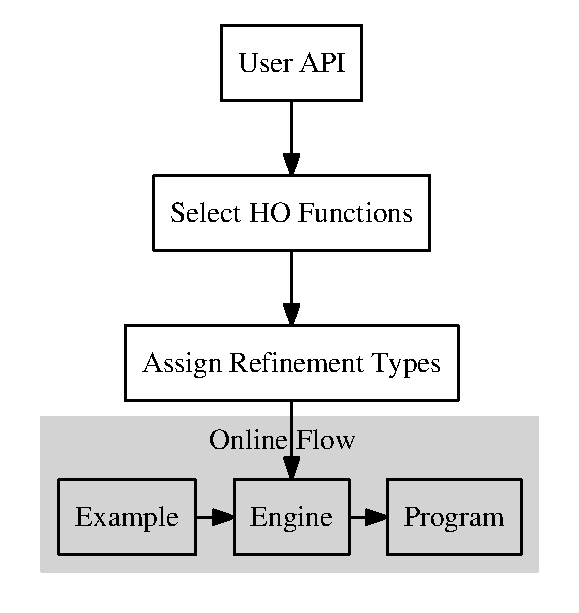
\includegraphics[width=0.4\textwidth]{algo}
  \caption{High-level structure of the algorithm.}
  \label{fig:high_level_overview}
\end{figure}

Figure~\ref{fig:high_level_overview} gives a high-level description of ways in which the components of our algorithm interact. Broadly speaking, there are two main stages in the algorithm. The offline (preprocessing) phase gathers the higher order declarations visible in the APIs and user-provided code, and assigns refinement types to them to build a custom synthesis \textit{engine}. This engine is then used during the online phase of the algorithm to search for functions that fit a set of supplied examples.

During the offline phase, the algorithm first scans the user-provided code, the libraries it imports, and the standard library to gather all of the functions and global values visible to the program. Then, it selects the higher-order functions from the set of all functions and values, and uses Liquid Haskell \cite{DBLP:conf/haskell/VazouSJ14, DBLP:conf/esop/VazouRJ13, DBLP:conf/icfp/VazouSJVJ14} to assign refinement types to each one. Finally, each higher-order function is assigned a weight based on locality\cite{insynthPLDI}. User-defined functions are given the highest priority, while direct imports are given less, and the standard libraries are given the least. Together with the first-order functions and values, these triples of higher-order functions with their refinement types and weights are collected to produce a synthesis engine.

Once this stage is complete, the user can examples to the synthesis engine, which will search the space of constructable functions for those that fit the examples. First, the engine computes a refinement type that fits the examples. This type is matched against the refinement types of the known higher-order functions, and the weights of each known function are adjusted based on how close the types match, if at all.

Once the candidate higher order functions have been chosen, the synthesis engine performs a best-first search for a program that fits all of the input and output examples by composing the candidates with first-order functions. For example, the higher-order function \texttt{map} might be supplied the \texttt{length} function if the example inputs are lists of lists of integers and the output examples are all lists of integers. The programs that are examined during the search are evaluated against the example set and are reported to the user as they match. Because the weights favor local declarations, the highest-ranked programs are likely to be the most idiomatic.

\markk{explain each of these lines in the rest of the paper, citing line numbers. once all of the lines are covered here we are done}
 We will explain each line of this in the proceeding Sections.
 
\begin{lstlisting}[caption=A pseudocode representation of the build and synthesis stages of the synthesis algorithm, label=listing:Algo]
main = do
  eng <- build
  ex  <- getExamples
  synth eng ex
  
build = do
  allTypes   <- collectTypesAndWeights
  allHOTypes <- filter isHigherOrder allTypes
  allRTypes  <- assignRTypes allHOTypes
  return (allTypes,allRTypes)
  
synth eng ex = do
  -- assign refinement types to examples
  exType   <- getExampleType ex
  exRType  <- assignRTypes exType
  -- make candidate functions and programs
  hoFxns <- rankByTypeMatch exRType eng
  progs  <- makeFxns exType hoFxns
  -- test the ranked list of possible programs
  validProgs <- filter (testOn ex) progs
\end{lstlisting}
